\documentclass[10pt,a4paper,twocolumn]{article}
% \usepackage{epcg_en}  % for English
\usepackage{epcg_pt}  % for Portuguese

\usepackage{graphicx}
\usepackage{subfig}
\usepackage{times}
%\usepackage{epsfig}

%\usepackage[T1]{fontenc}	% BETTER FONTS I GUESS
%\usepackage{ucs}
%\usepackage[utf8]{inputenc}
\usepackage[latin1]{inputenc}
\pagestyle{empty}
%\usepackage{pdfsync}

\title{Utiliza��o de Motion Tracking para Navega��o e \\Manipula��o de Objectos frente a Ecr� de Larga Escala}


% \author{Manuel J. Fonseca~~~~Joaquim A. Jorge \\
% Department of Information Systems and Computer Science \\
% INESC-ID/IST/Technical University of Lisbon \\
% R. Alves Redol, 9, 1000-029 Lisboa, Portugal \\
% \small{\texttt{mjf@inesc-id.pt, jorgej@acm.org}}}

\author{
\begin{tabular}{ccc}
	Jos� Pedro Dias & Jos� Gon�alves & Joaquim Jorge \\
	\multicolumn{2}{c}{Instituto Superior T�cnico} & INESC-ID \\
	\multicolumn{2}{c}{Av. Prof. Dr. Cavaco Silva} & R. Alves Redol, 9 \\
	\multicolumn{2}{c}{2744-016 Porto Salvo} & 1000-029 Lisboa \\
	\small{\texttt{jose.pedro.dias@gmail.com}} & \small{\texttt{jose.goncalves@ist.utl.pt}} & \small{\texttt{jaj@inesc.pt}}
\end{tabular}
}

%Jos� Pedro Dias\hspace{3cm}Jos� Gon�alves\hspace{3cm}Joaquim Jorge\\
%Instituto Superior T�cnico -- P�lo Tagus Park \\
%Av. Prof. Dr. Cavaco Silva, 2744-016 Porto Salvo \\
%\small{\texttt{jose.pedro.dias@ist.utl.pt\hspace{1.5cm}jose.goncalves@ist.utl.pt\hspace{1.5cm}jaj@inesc.pt}}}


%\date{}
\graphicspath{{figures/}}

% ABSTRACT
\chapter*{Abstract}
\addcontentsline{toc}{chapter}{Abstract}

\TODO{review and summarize this part, add implementation part.}

% context and problem
Nowadays the architectural project workflow is highly segmented
between the creative part and the CAD modeling part.
It starts with the architects drafting hand-made sketches of building designs
to study viable designs and validating them with clients, a stage without computer usage, 
with all participants on location using pen and paper.
Later on a set of documents is generated from the ground up on CAD software, 
using desktop computers and WIMP interfaces.

% motivation, goals
There's an increasing availability of alternative methods for both sketching, navigation and visualization
of 3D scenes which can enrich the design process and provide a better experience for both
building drafting, visualization and review.
We're committed to developing a multimodal distributed system to fulfill these goals
using tablet PCs or other devices facing a powerwall.
%We're committed to developing a multimodal system allowing multi-user scene navigation,
%building draft building designs, navigation and content reviewing.
It is thought out to integrate the architectural workflow as a creative and reviewing tool
to complement the early stages of architectural design.

% document organization
This survey begins with an analysis of projects with similar goals,
followed by a set of issues to handle:
how to get input from users,
display interactive content to them,
make shape creation and transformation possible and
allow scene navigation
%provide content reviewing capabilities.
A comparative analysis between architecture creation systems available in the market is then conducted and
finally conclusions are reached and directions for project execution defined.

\textbf{Keywords:} urban architecture, city, building, multimodal interaction, navigation, content reviewing


\begin{document}
\maketitle
\thispagestyle{empty}

\section{Introdu��o}

O prop�sito deste trabalho � o de permitir a utilizadores a execu��o de opera��es geom�tricas sobre
modelos tridimensionais.
As opera��es devem ser fornecidas ao utilizador de forma contextual, no pr�prio ambiente de visualiza��o,
fornecendo um conjunto de restri��es direccionais de modo a auxili�-lo a obter o efeito desejado.

A aplica��o de uma opera��o inicia-se com a selec��o atrav�s de um tra�o de uma face ou aresta a afectar,
o que despoleta o aparecimento de um menu contextual.
O utilizador escolhe ent�o a opera��o a aplicar, sendo esse mesmo tra�o interpretado para determina��o
dos par�metros da opera��o.

O sistema foi implementado como funcionalidade do prot�tipo multimodal ImmiView presente no laborat�rio Louren�o Fernandes
do IST Tagus Park \cite{leme}, permitindo a sua aplica��o em cen�rios com tablet PCs ou ecr�s de larga escala.

\begin{figure}[!ht]
	\centering
	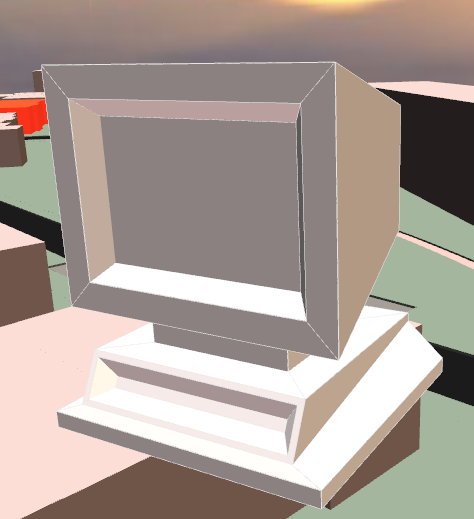
\includegraphics[width=0.4\linewidth]{ex-monitor.png}
	\vspace{-3mm}
	\caption{monitor modelado no sistema}
	\label{fig:example}
	\vspace{-3mm}
\end{figure}

\section{Interface com Utilizador}

A escolha de face opera-se pelo desenhar exclusivamente sobre a face.
A escolha de aresta opera-se cruzando a mesma, tendo in�cio numa das suas faces vizinhas e acabando na outra.
A figura \ref{fig:selection} ilustra este processo.


\begin{figure}[ht]
	\centering
	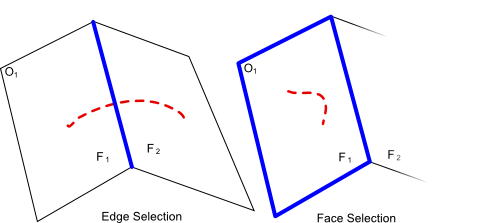
\includegraphics[width=0.9\linewidth]{face-edge-selection.png}
	\caption{selec��o de aresta ou face}
	\label{fig:selection}
\end{figure}

Uma vez escolhido o componente, um menu contextual surge, permitindo a escolha
de uma opera��o a aplicar (ver figura \ref{fig:contextual}).

\begin{figure}[!h]
	\centering
	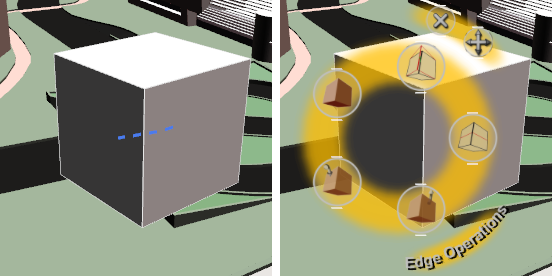
\includegraphics[width=0.75\linewidth]{contextual.png}
	\caption{activa��o de menu contextual de aresta}
	\label{fig:contextual}
\end{figure}

Em diversas opera��es suportadas um dos par�metros � a direc��o.
Quando assim �, um sistema de escolha de direc��o entra em funcionamento.
A direc��o do tra�o efectuado � comparada com os diversos sugeridos, aplicando-se
a que mais se aproximar do mesmo (ver figura \ref{fig:election}).
Este mecanismo � denominado no software da especialidade como \textit{snapping}.

\begin{figure}[!h]
	\centering
	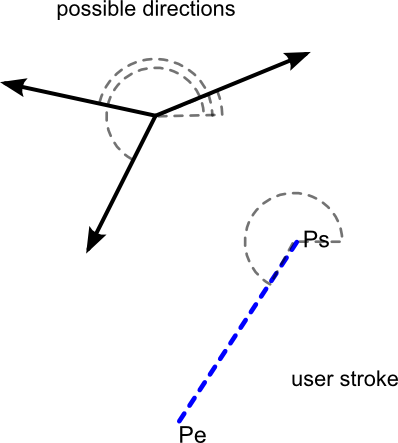
\includegraphics[width=0.35\linewidth]{election.png}
	\caption{elei��o do vector mais pr�ximo}
	\label{fig:election}
\end{figure}

%A figura \ref{fig:icons} lista as opera��es suportadas e respectivos �cones.
%
%\begin{figure}[ht]
%	\centering
%	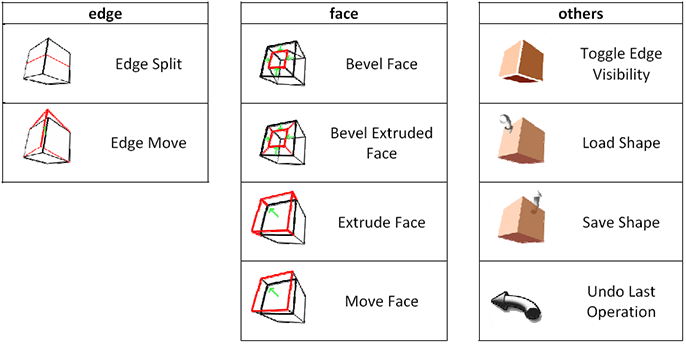
\includegraphics[width=0.94\linewidth]{icons.png}
%	\label{fig:icons}
%	\caption{opera��es dispon�veis por menu e respectivos �cones}
%\end{figure}

\section{Opera��es Suportadas}

Segue-se a descri��o de direc��es suportadas pelas opera��es, como ilustrado
na figura \ref{fig:shots}.

\subsection{Altera��o da Geometria}

\textbf{Extrus�o} --
direc��o definida pela compara��o com as normais da face origem.
Comprimento baseado no comprimento do tra�o.


\textbf{Bevel} --
a dimens�o do \textit{bevel} � dependente do comprimento do tra�o.


\textbf{Mover Face} --
suporta n�o s� as direc��es normais como tamb�m as co-lineares com as arestas fronteira da face.


\textbf{Mover Aresta} --
suporta as normais � aresta e as direc��es das faces vizinhas da mesma.


\textbf{Corte de Aresta} --
processa-se imediatamente, propagando o corte por arestas opostas at� terminar o \textit{loop} de face.

\subsection{Outras opera��es}

\textbf{Anular Opera��o} --
todas as opera��es desde a instancia��o do objecto podem ser revertidas.

\textbf{Salvaguarda e carregamento} --
o objecto pode ser guardado num formato simples em XML.
A exporta��o de conte�do a partir de pacotes de modela��o � poss�vel,
tendo sido implementado um \textit{plug-in} para Blender.

\begin{figure}[!ht]
	\centering
	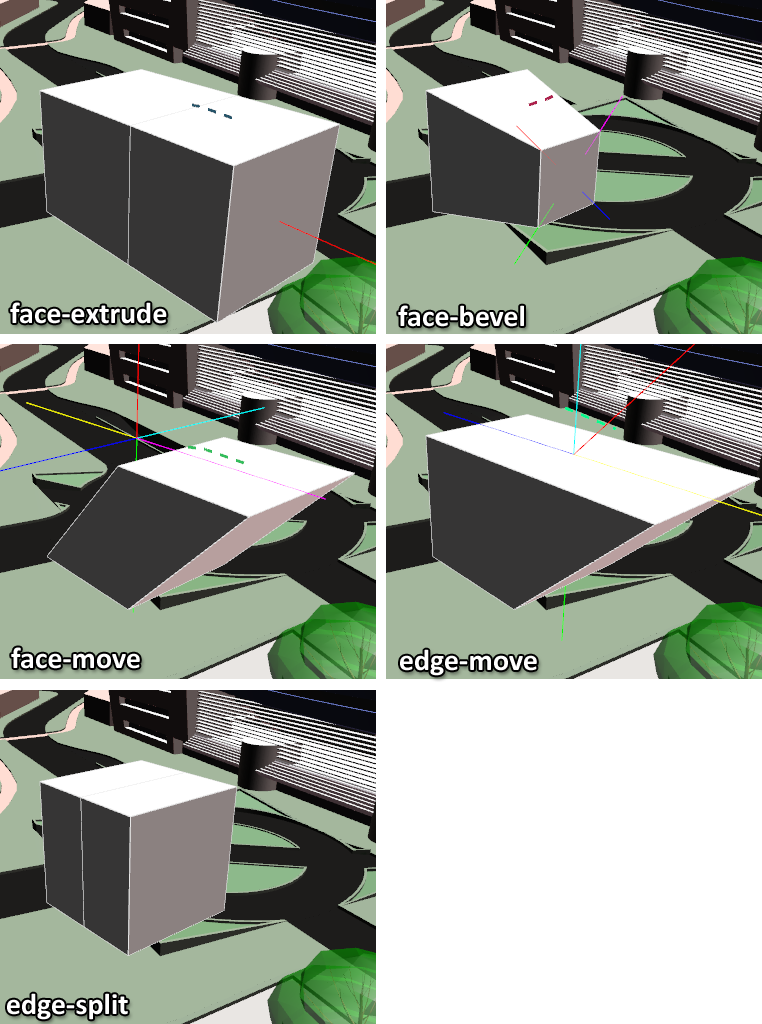
\includegraphics[width=0.8\linewidth]{shots2.png}
	\vspace{-3mm}
	\caption{opera��es no ImmiView}
	\label{fig:shots}
	\vspace{-3mm}
\end{figure}

\section{Representa��o Interna}

A estrutura do modelo geom�trico proposta � baseada em faces de 4 v�rtices. 
Esta estrutura implica que:
cada aresta seja partilhada por duas faces;
cada aresta pertencente a uma face tenha uma face oposta.

Al�m de guardar a lista de v�rtices e respectivas posi��es, assim como a lista de faces
(uma face � uma lista de quatro �ndices de v�rtices), � gerada uma estrutura auxiliar,
o mapa de arestas, que associa a cada aresta as faces que lhe s�o vizinhas. Esta informa��o
vai permitir o c�lculo de diversos vectores auxiliares assim como tornar poss�vel a opera��o
de corte de \textit{loop} de faces.

%Outras estruturas s�o igualmente definidas, como um lista de cores ou materiais por face.

O mecanismo de \textit{undo} foi implementado, baseado no padr�o de desenho Memento \cite{despat}.
Cada objecto tem associada uma pilha de estados de modo a poder regressar a qualquer passo anterior de modela��o.

A persist�ncia de objectos recorre a uma estrutura simples em XML, como se ilustra:

%\textbf{Salvaguarda e Carregamento} --
%uma forma geom�trica pode ser guardada para posterior carregamento num formato
%XML definido. O mesmo segue o seguinte padr�o:
\begin{scriptsize}
	\begin{verbatim}
	<?xml version="1.0" encoding="utf-8"?>
	  <shape>
	    <vertices count="56">
	      <vertex x="-1" y="-0.627882" z="5.29942"/>
	      ...
	    </vertices>
	  <faces count="54">
	    <face v1="0" v2="1" v3="2" v4="3"/>
	    ...
	  </faces>
	  <colors count="54">
	    <color r="0.9" g="0.9" b="0.9"/>
	    ...
	  </colors>
	</shape>
	\end{verbatim}
\end{scriptsize}

\section{Conclus�es e Trabalho Futuro}

O projecto iniciou-se com uma cuidada defini��o do mesmo,
a elabora��o abstracta das estrutura e algoritmos necess�rios,
execu��o de um 1� prot�tipo Java para validar as mesmas
e posterior adapta��o ao projecto ImmiView.

A inclus�o neste projecto trouxe suporte
para detec��o de tra�os e menus circulares contextuais,
o que permitiu oferecer um mecanismo simples e eficiente de
invocar opera��es geom�tricas sobre formas tridimensionais.

Est�o agendados testes com utilizadores para o final de Setembro de 2007.
Esta solu��o de modela��o ser� parte integrante de um sistema de cria��o
de paisagens urbanas desenvolvido pelo autor.

%Incialmente nao estava comentado
% \nocite{*}

\bibliography{epcg}
\bibliographystyle{long_pt} % for portuguese
% \bibliographystyle{long_en} % for english
\end{document}